% 06-validation.tex — Validation par rapport aux formules du cours, limites.

\section{Validation et limites}
\label{sec-validation}

La simulation doit donner raison aux formules du cours, sinon le jeu
contredirait l'exercice. Trois comparaisons ont été faites avec le code du
site (\texttt{outils/donnees.mjs}).

\paragraph{Seuil de l'eau.} Pour 24 configurations (4 lieux,
\(L = \num{0,2}\), \num{0,4} et \SI{0,6}{m}, \(m = 1\) et \SI{5}{kg}), le
seuil de réussite, trouvé par dichotomie sur \(v_0\), vaut
\(v_0^\star = k \sqrt{5 g R}\) avec \(k\) entre \num{0,92} et \num{0,97}, élan
compris. Le seuil est un peu sous la valeur théorique pour deux raisons. D'une
part, le seau passe le point bas un peu plus vite que \(v_0\) : de 3 à
\SI{7}{\percent} sur les cinq configurations du \cref{tab-tours}, car
l'alignement apporte encore un peu d'énergie et la barre et la corde, lancées
avec le seau, cèdent la leur. D'autre part, l'eau est plus loin du pivot que le
centre de masse du seau, et la rotation du seau la plaque un peu plus au fond :
elle demande un peu moins que \(5 g R\).

\paragraph{Tension.} Pendant les tours libres, la tension simulée suit la
forme de l'équation~\eqref{eq-tension}, avec un maximum au point bas et un
minimum au sommet (\cref{fig-tension}). Son pic dépasse
\(m (v_0^2/R + g)\) de 11 à \SI{33}{\percent} (\cref{tab-tours}). L'excès de
vitesse en explique une partie ; la masse de la corde explique le reste, et
c'est pour un seau léger au bout d'une longue corde que l'écart est le plus
grand. La borne haute de la fenêtre garantie inclut déjà la charge propre de la
corde, et le facteur \num{0,8} laisse en plus \SI{25}{\percent} de marge
(\(1/\num{0,8}\)), qui couvre l'excès dû à la vitesse ; le cas à
\SI{33}{\percent} (\(m = \SI{0,5}{kg}\), \(L = \SI{0,6}{m}\)) est hors des
tirages du jeu.

\begin{figure}[!htb]
  \centering
  \begin{subfigure}[b]{0.49\linewidth}
    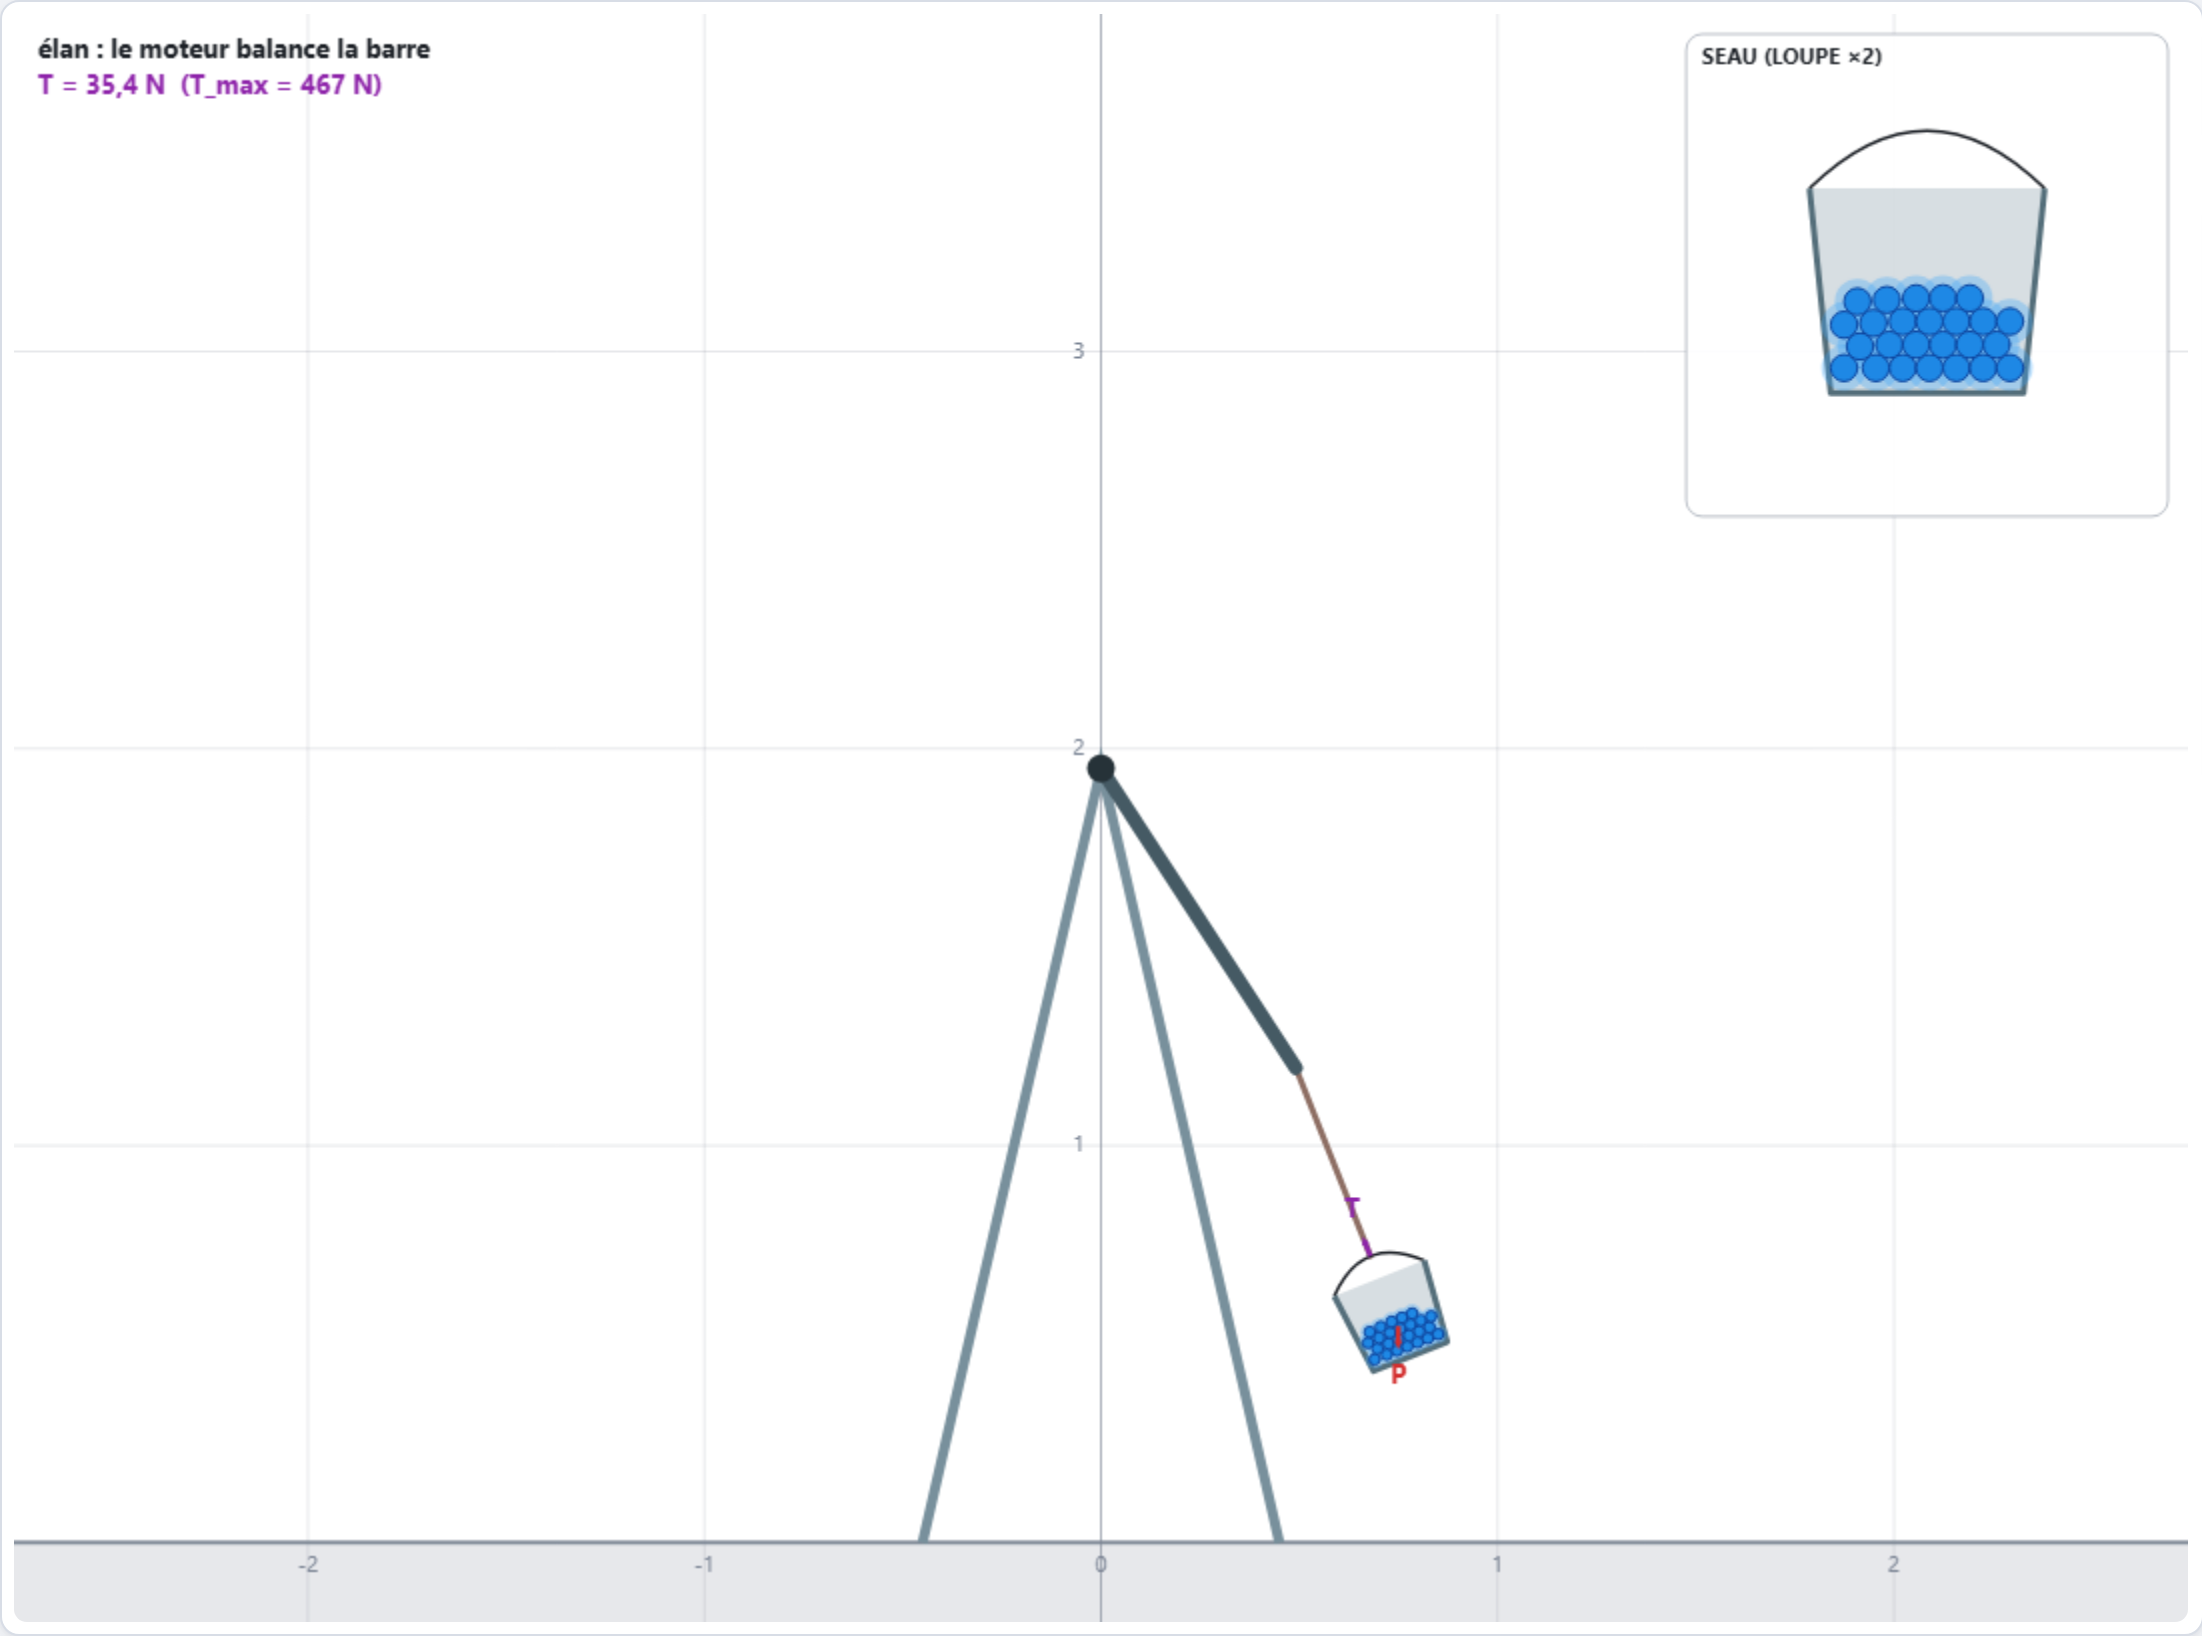
\includegraphics[width=\linewidth]{captures/jeu-elan.png}
    \caption{Élan : va-et-vient au rythme du pendule.}
  \end{subfigure}\hfill
  \begin{subfigure}[b]{0.49\linewidth}
    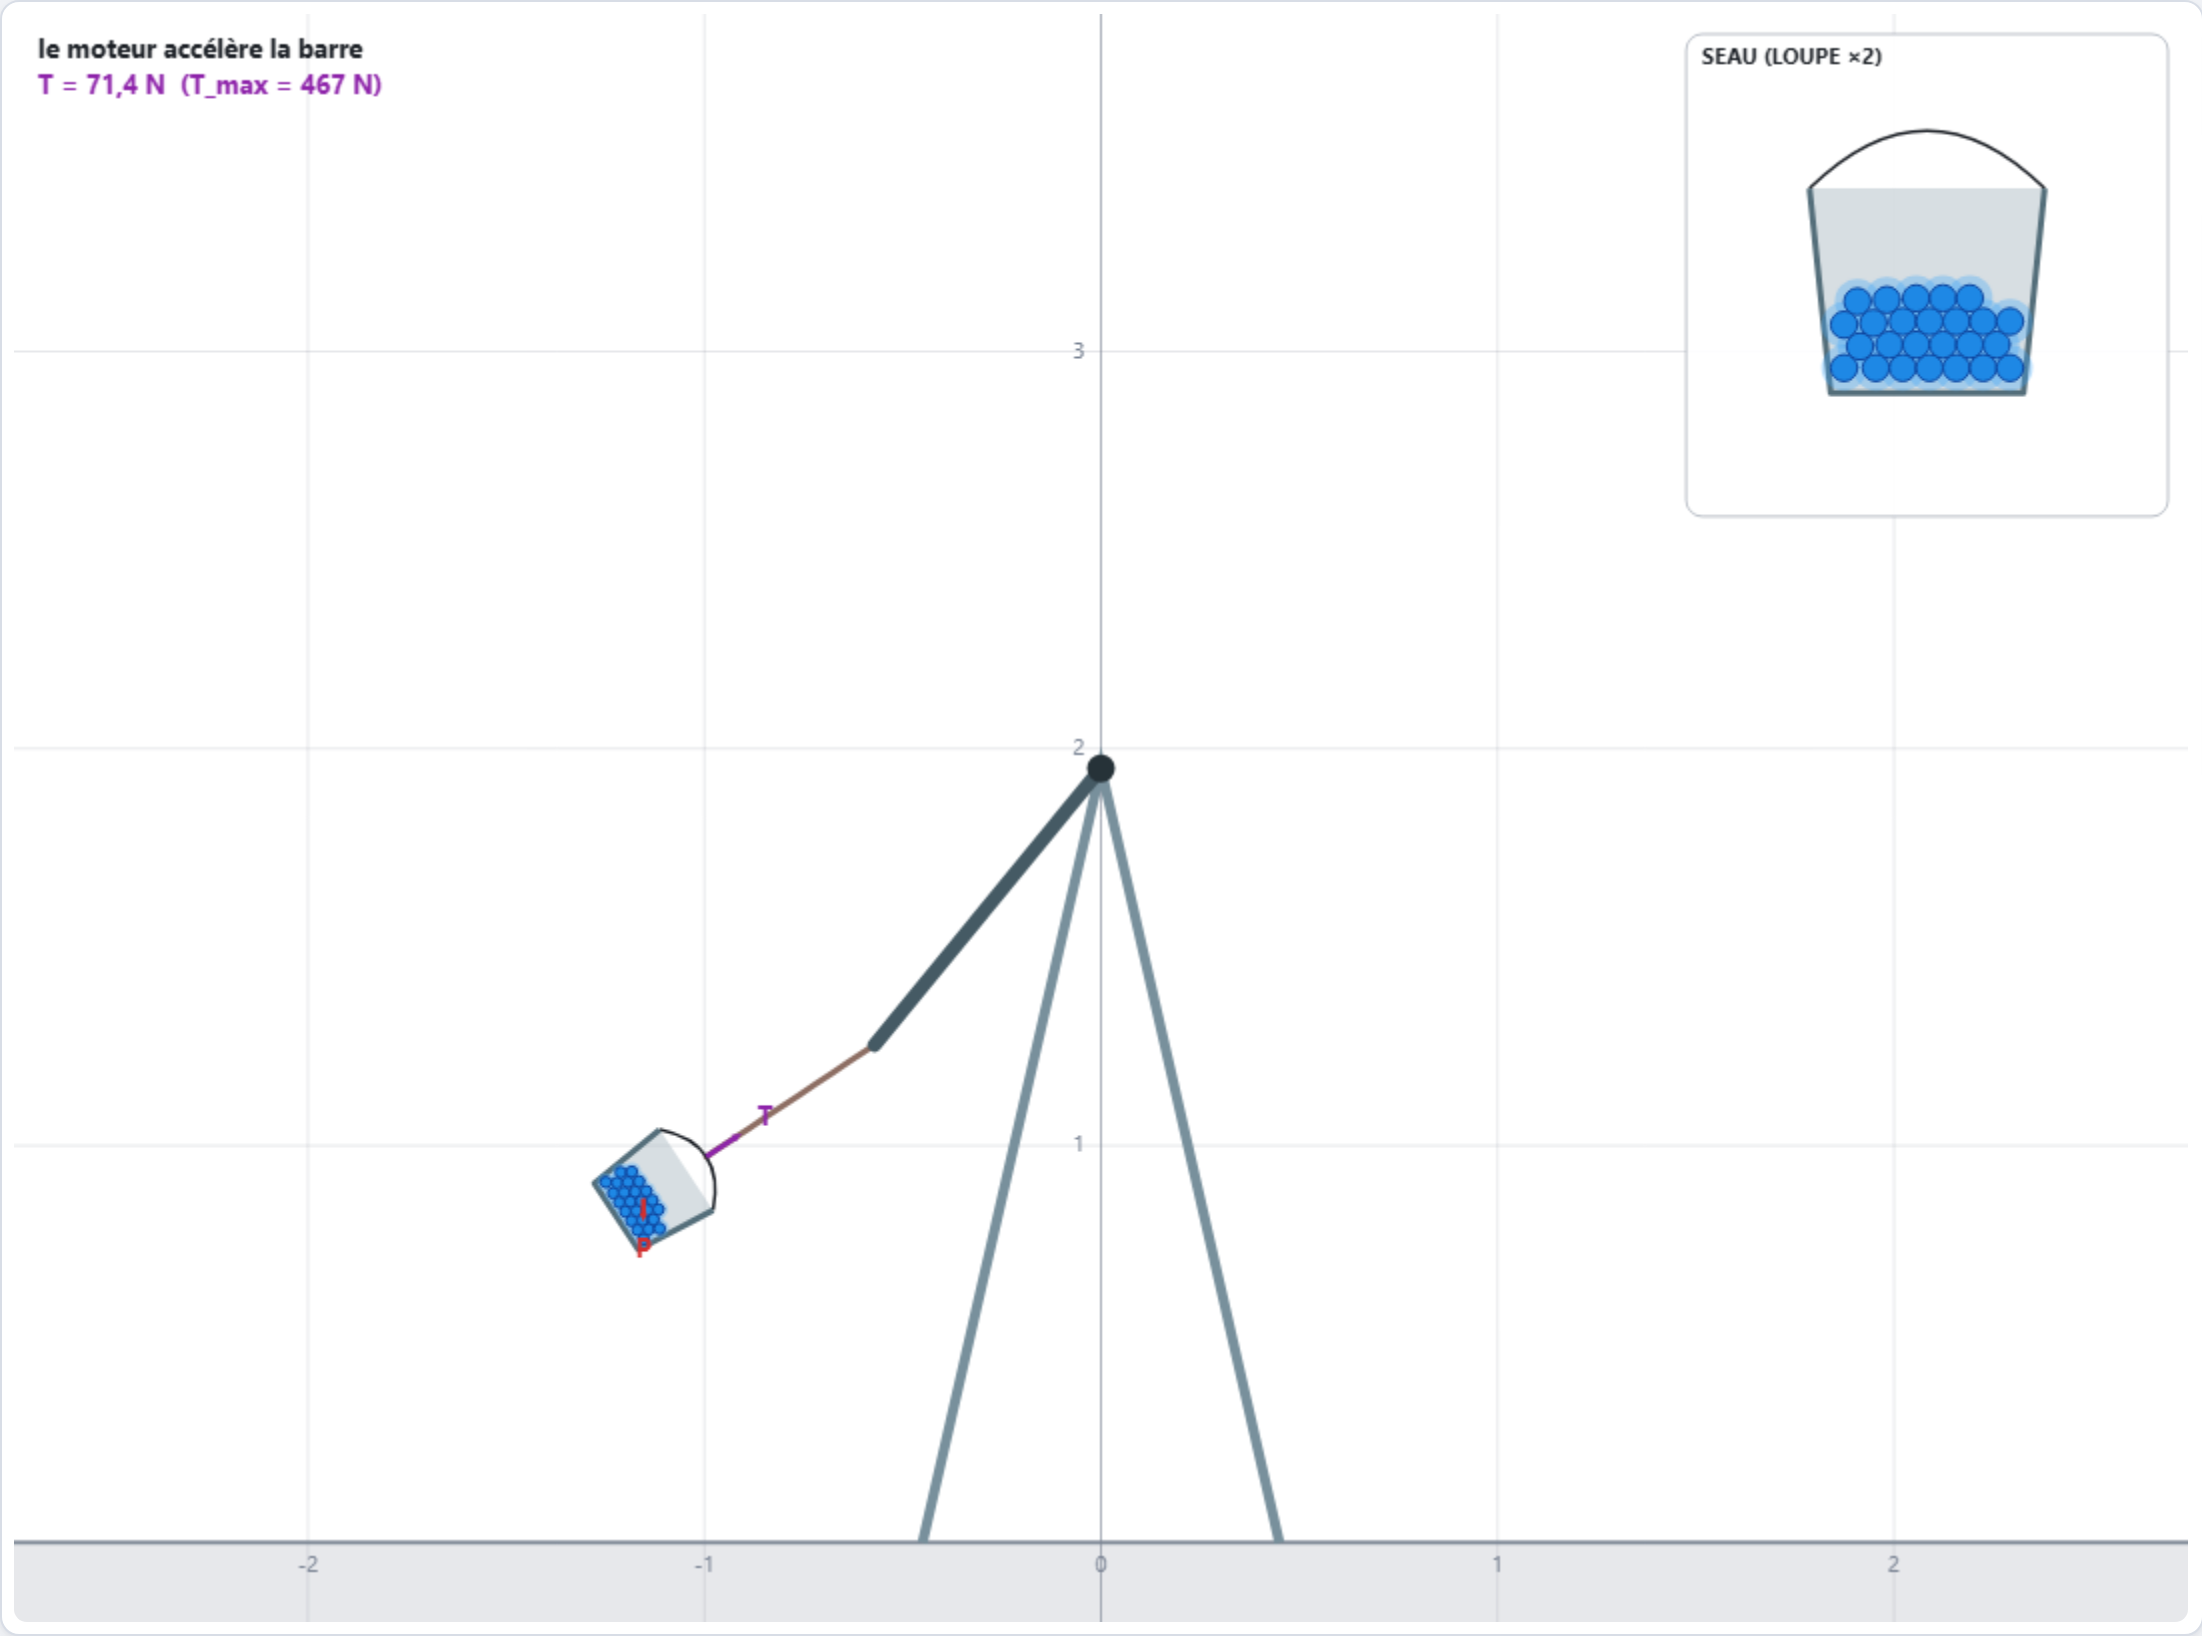
\includegraphics[width=\linewidth]{captures/jeu-lancer.png}
    \caption{Lancer : la barre devance le seau, la corde tire en biais.}
  \end{subfigure}\\[4pt]
  \begin{subfigure}[b]{0.49\linewidth}
    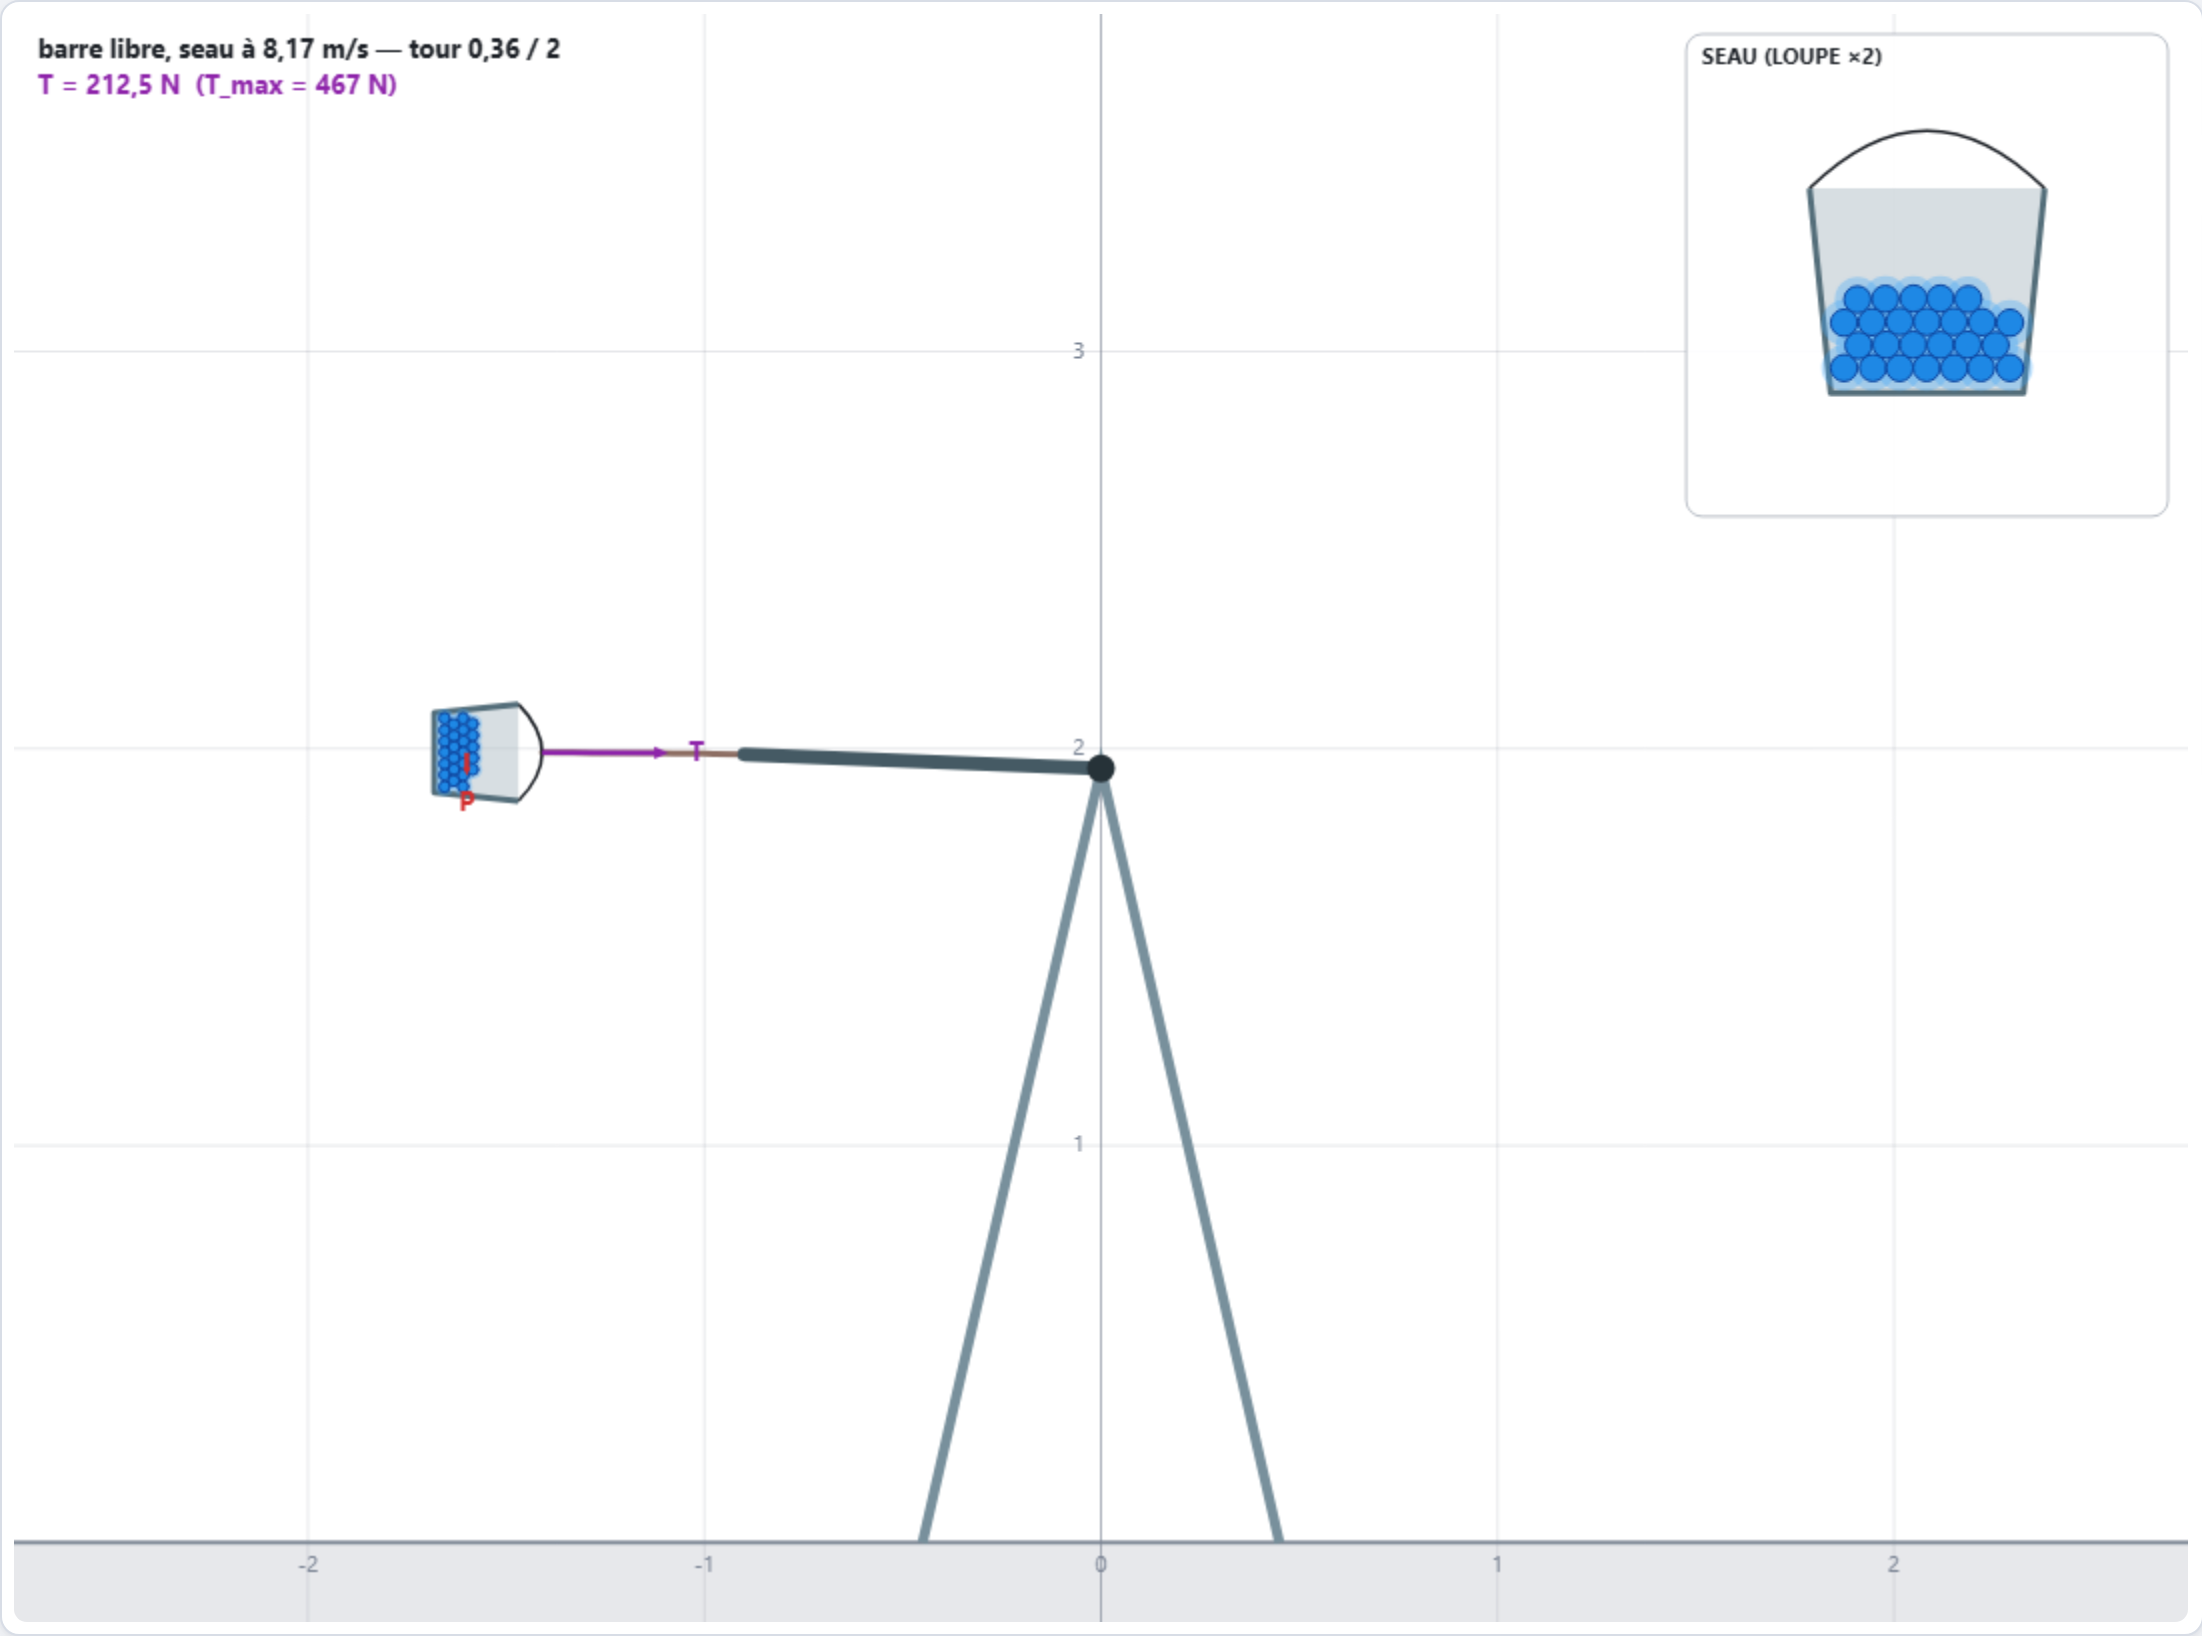
\includegraphics[width=\linewidth]{captures/jeu-tour-libre.png}
    \caption{Tour libre : chaîne alignée, eau plaquée au fond (loupe).}
  \end{subfigure}\hfill
  \begin{subfigure}[b]{0.49\linewidth}
    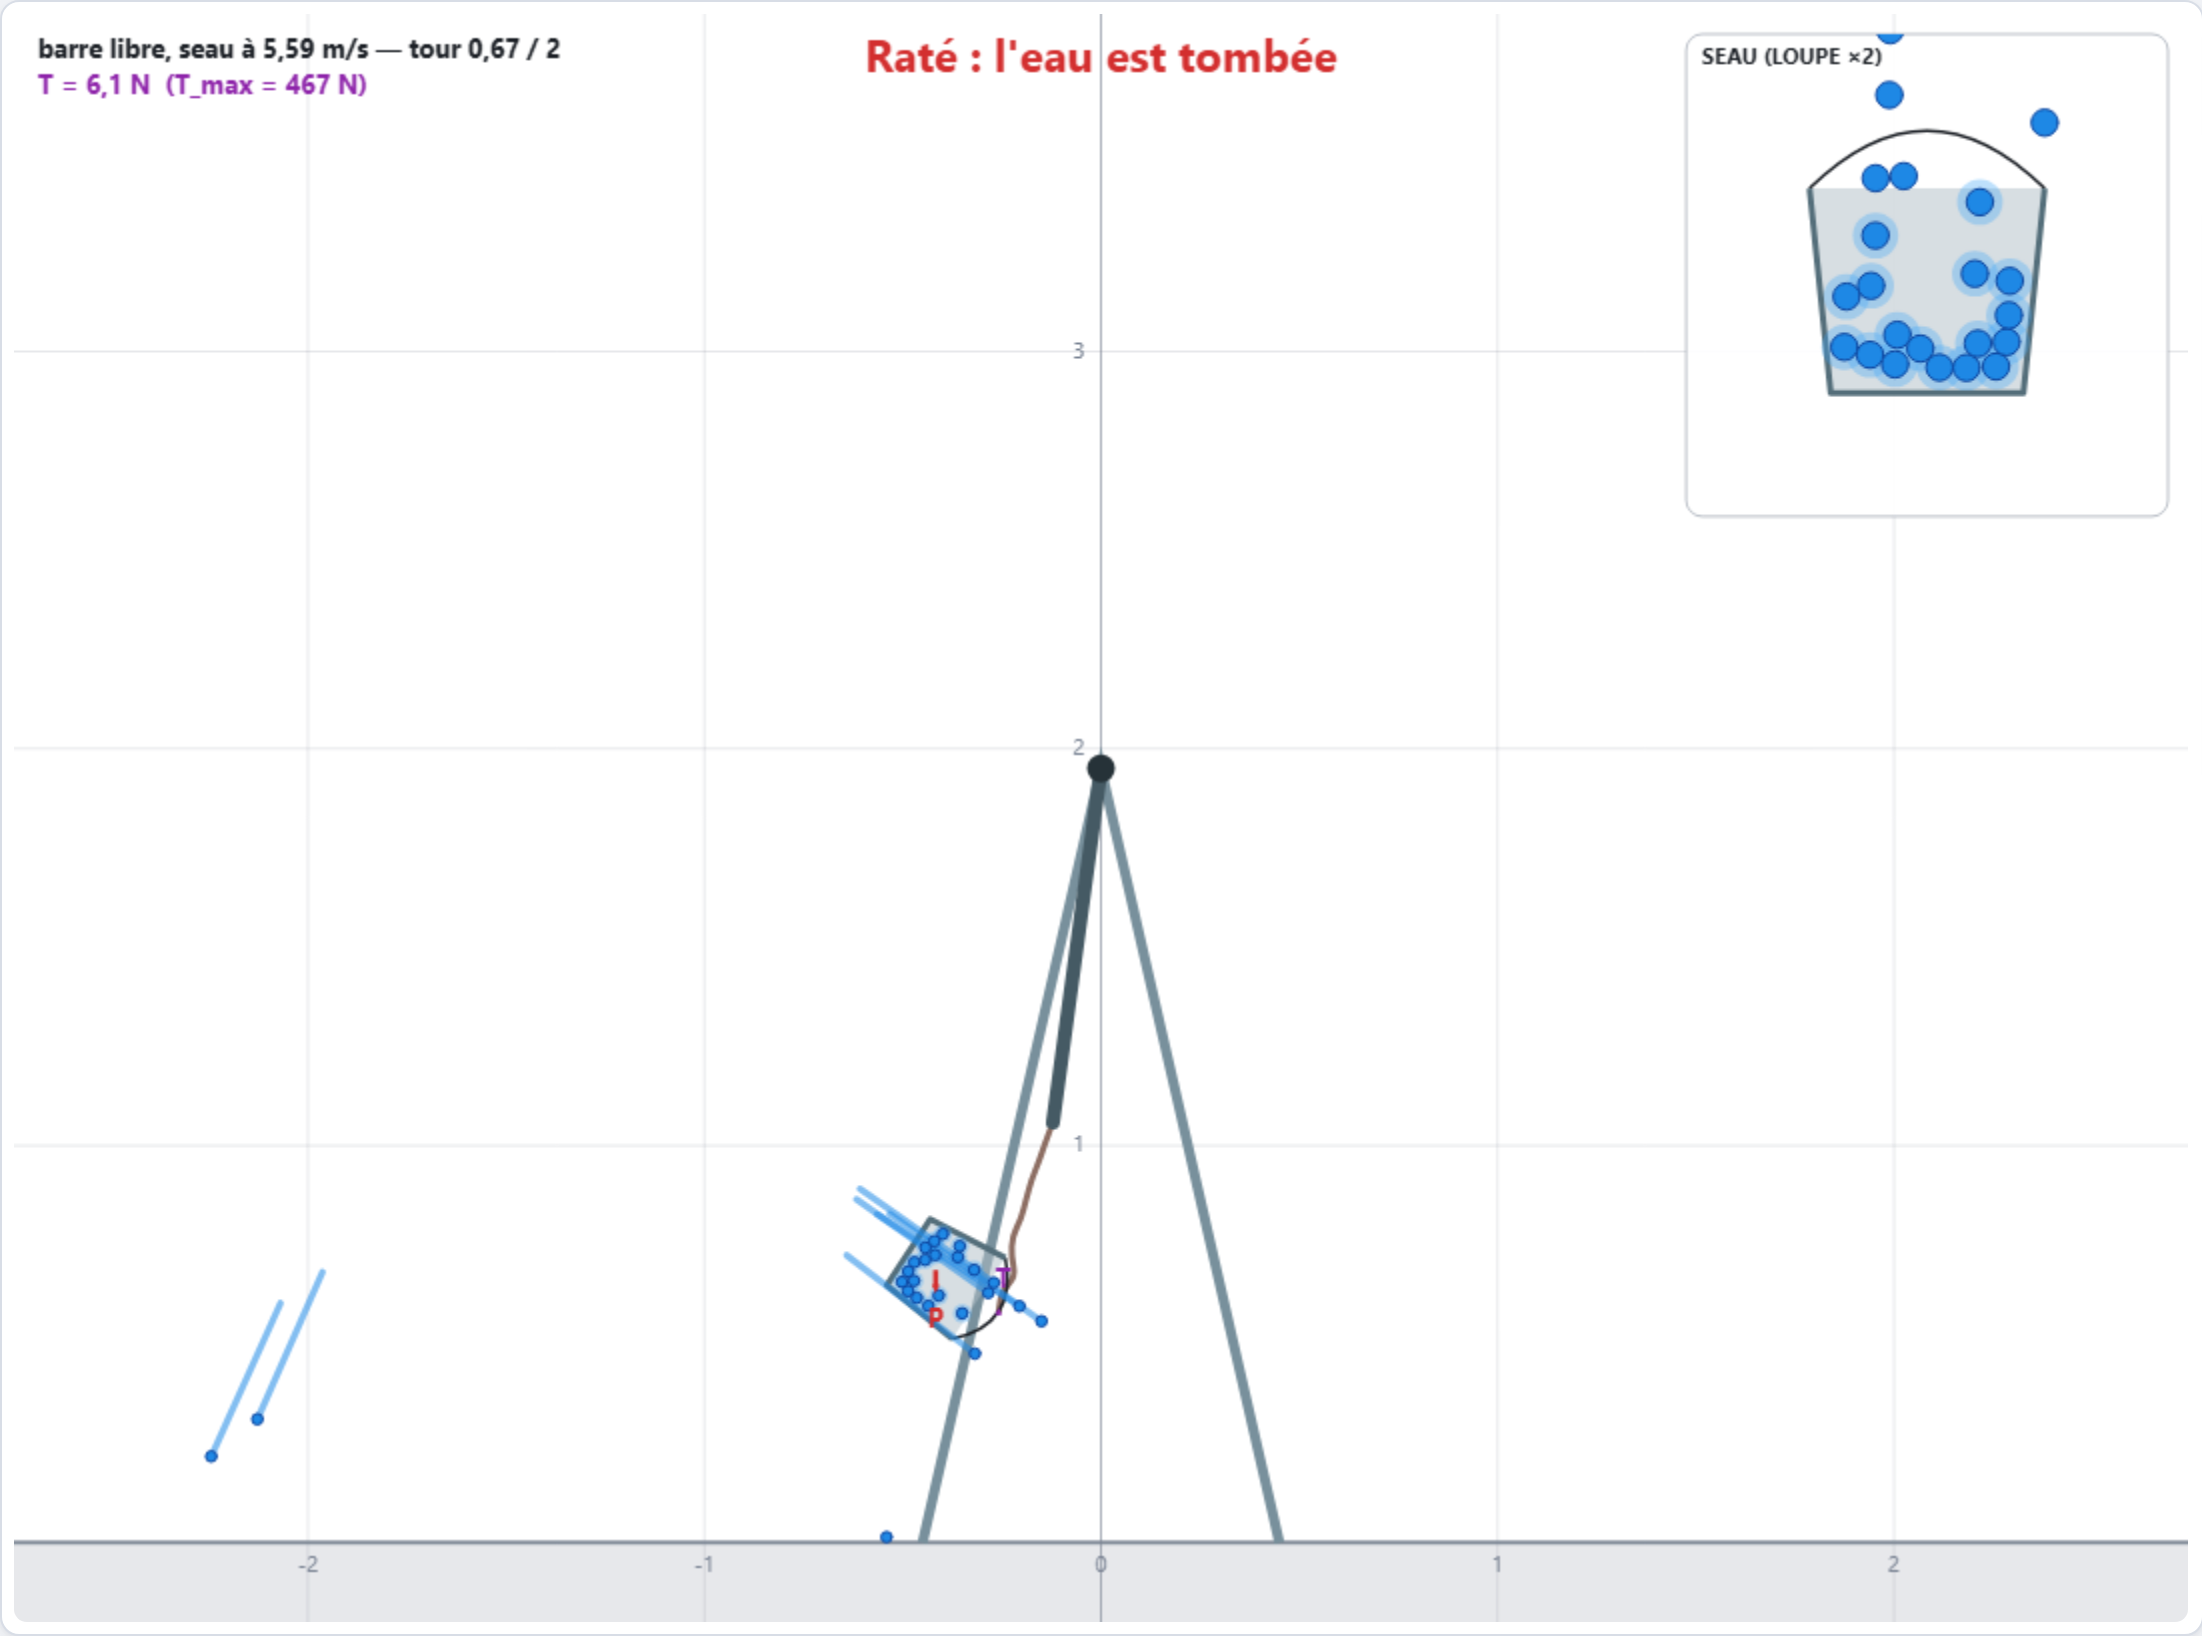
\includegraphics[width=\linewidth]{captures/jeu-rate.png}
    \caption{\(v_0 = 0{,}9 \sqrt{5 g R}\) : la corde se détend, l'eau tombe.}
  \end{subfigure}
  \caption{Captures du jeu (Terre, \(L = \SI{0,51}{m}\), \(m = \SI{4}{kg}\),
    \(T_{\max} = \SI{467}{N}\), fenêtre garantie \num{9,39} à
    \SI{11,47}{m/s}). Les vignettes (a) à (c) : \(v_0 = \SI{10,43}{m/s}\),
    réussi. En haut à droite, la loupe montre le seau dans son propre repère.}
  \label{fig-captures}
\end{figure}

\begin{figure}[!htb]
  \centering
  \begin{tikzpicture}
    \begin{axis}[width=0.78\linewidth, height=4.4cm, xlabel={\(t\) depuis le lâcher (s)}, ylabel={\(T\) (N)},
      xmin=0, grid=major, /pgf/number format/use comma, grid style={gray!20}, legend style={font=\scriptsize, at={(0.5,1.03)}, anchor=south, legend columns=2, draw=none},
      tick label style={font=\scriptsize}, label style={font=\small}]
      \addplot[tensionc, thick] table[x=t, y=simulee, col sep=comma] {figures/donnees/tension_seau.csv};
      \addplot[black, dashed] table[x=t, y=ideale, col sep=comma] {figures/donnees/tension_seau.csv};
      \legend{{simulée}, {\(m (v_0^2/R + g (3 \cos(\theta) - 2))\)}}
    \end{axis}
  \end{tikzpicture}
  \caption{Tension de la corde pendant les deux tours libres, comparée à
    l'équation~\eqref{eq-tension} (Terre, \(L = \SI{0,4}{m}\),
    \(m = \SI{2}{kg}\), \(v_0 = 1{,}15 \sqrt{5 g R} = \SI{9,83}{m/s}\)). La
    courbe idéale utilise \(v_0\) ; l'écart vient surtout de l'excès de vitesse
    au point bas et de la masse de la corde.}
  \label{fig-tension}
\end{figure}

\begin{table}[!htb]
  \centering
  \small
  \begin{tabular}{rrrrrr}
    \toprule
    \(g\) (\si{m/s^2}) & \(L\) (\si{m}) & \(m\) (\si{kg}) & \(v_0\) (\si{m/s}) & \(v_{\text{bas}}/v_0\) & \(T_{\text{pic}}/\left(m (v_0^2/R + g)\right)\) \\
    \midrule
    \num{9,81} & \num{0,2} & 5   & \num{9,55}  & \num{1,051} & \num{1,11} \\
    \num{9,81} & \num{0,4} & 2   & \num{10,26} & \num{1,057} & \num{1,15} \\
    \num{9,81} & \num{0,6} & \num{0,5} & \num{10,93} & \num{1,073} & \num{1,33} \\
    \num{3,71} & \num{0,4} & 2   & \num{6,31}  & \num{1,060} & \num{1,16} \\
    \num{1,62} & \num{0,6} & 1   & \num{4,44}  & \num{1,034} & \num{1,22} \\
    \bottomrule
  \end{tabular}
  \caption{Premier passage au point bas et pic de tension après le lâcher, pour
    \(v_0 = 1{,}2 \sqrt{5 g R}\) (vitesse estimée sur les images à
    \SI{60}{Hz}).}
  \label{tab-tours}
\end{table}

\paragraph{Limites.} Le modèle est plan, sans frottement au pivot ni résistance
de l'air. L'eau n'a pas de pression, sa viscosité est une simple traînée, et
elle ne réagit pas sur le seau ; un fluide plus réaliste (SPH ou fluides basés
sur les positions \cite{monaghan1992sph, macklin2013pbf}) n'apporterait rien à
la question posée à l'étudiant : à quelle vitesse l'eau reste-t-elle dans le
seau ? Le seau passe le point bas 3 à \SI{7}{\percent} plus vite que \(v_0\) :
le jeu est un peu plus tolérant que la formule pour la borne basse, mais plus
sévère pour la borne haute, où la tension simulée dépasse la formule. C'est
pourquoi la fenêtre garantie n'utilise que \SI{80}{\percent} de \(T_{\max}\) ;
les cinq valeurs qu'en rejoue le vérificateur réussissent toutes. Enfin,
un départ plus brutal, qui montrerait davantage la corde molle et les
éclaboussures, a été essayé : il fait tomber l'eau quel que soit \(v_0\), ce qui
rendrait les défis insolubles. Il n'a donc pas été retenu.


\FloatBarrier

\section{Conclusion}

Le jeu reproduit la condition \(v_0^2 \geq 5 g R\) du cours à 3 à
\SI{8}{\percent} près (\(k = \num{0,92}\) à \num{0,97}) avec une corde qui plie
et de l'eau en particules, sans autre action sur le seau que son poids et la
corde. Chaque défi tiré est vérifié en rejouant la simulation, et les écarts
restants (vitesse au point bas, masse de la corde, taille du seau) sont
expliqués et couverts par les marges de la fenêtre garantie.
